\documentclass{article}

\usepackage[T1]{fontenc}
\usepackage{graphicx}
\usepackage{fancyhdr}
\pagestyle{fancy}
\fancyhf{}
\lhead{Version 2.0}
\rhead{Elliot Oram}
\rfoot{\thepage}


\title{Website design}
\author{elo9@aber.ac.uk}

\begin{document}

\maketitle
\tableofcontents

\newpage

\section{Website design diagram}
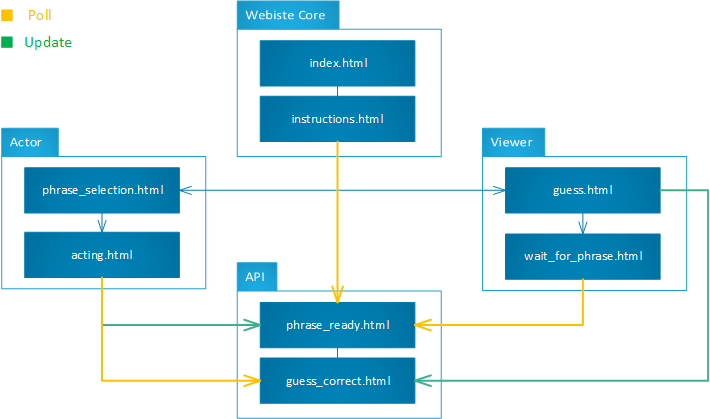
\includegraphics[width=\textwidth]{WebsiteDesign.png}


\section{Description of Website design}
\subsection{Core}
\begin{itemize}
	\item \textbf{index.html}: The main landing page for the webapp. This will contain an input for the session id that will be used to keep track of the users and will have the option to select either an actor or viewer as the user type.
	
	\item \textbf{instructions.html}: This page will display the instructions on how to play the game. The page contents will differ depending on the user type. The instructions page polls the phrase\_ready.html api page and when it is ready the page will refresh and display the continue buttons for the viewers. 
\end{itemize}


\subsection{Actor}

\begin{itemize}
	\item \textbf{phrase\_selection.html}: Allows the actor to select the phrase that they wish to act out. The actor will be given the opportunity to choose from a list of five different phrases.
	
	\item \textbf{acting.html}: This page will show the current word that the actor is acting and a timer for how long they have remaining. This page when initially loaded, and when a word is selected, will update the phrase\_ready api which will allow the viewers to start guessing. The page will then poll the guess\_correct.html api to discover if the word that is being acted has been successfully guessed. If it has then the phrase\_ready will be is updated to False, and the Actor is redirect back to the phrase\_selection page. 
	
\end{itemize}


\subsection{Viewer}

\begin{itemize}
	\item \textbf{guess.html}: This page will display information about what the actor is acting to the user. The information will include the topic or genre, the current word in the phrase being acted (e.g. word number 3 of 5), the number of letters in that word, and how long until the round ends. If the viewer guesses correctly, this will update the guess\_correct.html api to True and move all viewers to the wait\_for\_phrase.html page.
	
	\item \textbf{wait\_for\_phrase.html}: This page is a waiting zone for the users while the actor selects a new phrase. This page polls the phrase\_ready api and will redirect users when the phrase is ready to be guessed.
	
\end{itemize}

\subsection{API}

\begin{itemize}

	\item \textbf{phrase\_ready.html}: Returns a boolean for if the phrase is ready to be guessed by the viewer.
	
	\item \textbf{guess\_correct.html}: Returns a boolean for if the phrase has been guessed correctly by the viewer.

\end{itemize}
 
\end{document}